%%
%% Automatically generated file from DocOnce source
%% (https://github.com/hplgit/doconce/)
%%
%%
% #ifdef PTEX2TEX_EXPLANATION
%%
%% The file follows the ptex2tex extended LaTeX format, see
%% ptex2tex: http://code.google.com/p/ptex2tex/
%%
%% Run
%%      ptex2tex myfile
%% or
%%      doconce ptex2tex myfile
%%
%% to turn myfile.p.tex into an ordinary LaTeX file myfile.tex.
%% (The ptex2tex program: http://code.google.com/p/ptex2tex)
%% Many preprocess options can be added to ptex2tex or doconce ptex2tex
%%
%%      ptex2tex -DMINTED myfile
%%      doconce ptex2tex myfile envir=minted
%%
%% ptex2tex will typeset code environments according to a global or local
%% .ptex2tex.cfg configure file. doconce ptex2tex will typeset code
%% according to options on the command line (just type doconce ptex2tex to
%% see examples). If doconce ptex2tex has envir=minted, it enables the
%% minted style without needing -DMINTED.
% #endif

% #define PREAMBLE

% #ifdef PREAMBLE
%-------------------- begin preamble ----------------------

\documentclass[%
oneside,                 % oneside: electronic viewing, twoside: printing
final,                   % draft: marks overfull hboxes, figures with paths
10pt]{article}

\listfiles               %  print all files needed to compile this document

\usepackage{relsize,makeidx,color,setspace,amsmath,amsfonts,amssymb}
\usepackage[table]{xcolor}
\usepackage{bm,ltablex,microtype}

\usepackage[pdftex]{graphicx}

\usepackage[T1]{fontenc}
%\usepackage[latin1]{inputenc}
\usepackage{ucs}
\usepackage[utf8x]{inputenc}

\usepackage{lmodern}         % Latin Modern fonts derived from Computer Modern

% Hyperlinks in PDF:
\definecolor{linkcolor}{rgb}{0,0,0.4}
\usepackage{hyperref}
\hypersetup{
    breaklinks=true,
    colorlinks=true,
    linkcolor=linkcolor,
    urlcolor=linkcolor,
    citecolor=black,
    filecolor=black,
    %filecolor=blue,
    pdfmenubar=true,
    pdftoolbar=true,
    bookmarksdepth=3   % Uncomment (and tweak) for PDF bookmarks with more levels than the TOC
    }
%\hyperbaseurl{}   % hyperlinks are relative to this root

\setcounter{tocdepth}{2}  % levels in table of contents

% Tricks for having figures close to where they are defined:
% 1. define less restrictive rules for where to put figures
\setcounter{topnumber}{2}
\setcounter{bottomnumber}{2}
\setcounter{totalnumber}{4}
\renewcommand{\topfraction}{0.95}
\renewcommand{\bottomfraction}{0.95}
\renewcommand{\textfraction}{0}
\renewcommand{\floatpagefraction}{0.75}
% floatpagefraction must always be less than topfraction!
% 2. ensure all figures are flushed before next section
\usepackage[section]{placeins}
% 3. enable begin{figure}[H] (often leads to ugly pagebreaks)
%\usepackage{float}\restylefloat{figure}

% prevent orhpans and widows
\clubpenalty = 10000
\widowpenalty = 10000

% --- end of standard preamble for documents ---


% insert custom LaTeX commands...

\raggedbottom
\makeindex
\usepackage[totoc]{idxlayout}   % for index in the toc
\usepackage[nottoc]{tocbibind}  % for references/bibliography in the toc

%-------------------- end preamble ----------------------

\begin{document}

% matching end for #ifdef PREAMBLE
% #endif

\newcommand{\exercisesection}[1]{\subsection*{#1}}


% ------------------- main content ----------------------



% ----------------- title -------------------------

\thispagestyle{empty}

\begin{center}
{\LARGE\bf
\begin{spacing}{1.25}
Electromagnetic braking
\end{spacing}
}
\end{center}

% ----------------- author(s) -------------------------

\begin{center}
{\bf Bror Hjemgaard, René Ask and Sigurd Sørlie Rustad${}^{}$} \\ [0mm]
\end{center}

\begin{center}
% List of all institutions:
\end{center}
    
% ----------------- end author(s) -------------------------

% --- begin date ---
\begin{center}
Jul 28, 2020
\end{center}
% --- end date ---

\vspace{1cm}


Many of you may be familiar with the experiment of dropping a magnet through a non-magnetic, conductive metal pipe. In this exercise we are going to study the unexpected motion of the falling magnet.

\section{Equipment list}
\label{title:equip_list}
Make sure you have all the equipment needed to do the experiment.
\begin{itemize}
  \item Aluminum foil tube

  \item Magnets

  \item Scale

  \item Stopwatch (Smartphone)

  \item Tape-measure or ruler
\end{itemize}

\noindent
\section{Understanding the experiment}
Imagine dropping a cylindrical magnet of mass $m$, radius $r$ and height $l$ vertically through the center of a non-magnetic, conductive metal ring. In Figure~\ref{fig:fallingmagnet}, the motion of the magnet is depicted at three different positions.

(a) The magnet is above the ring.

(b) The magnet is at the center of the ring.

(c) The magnet is below the ring.


\begin{figure}[!ht]  % fig:fallingmagnet
  \centerline{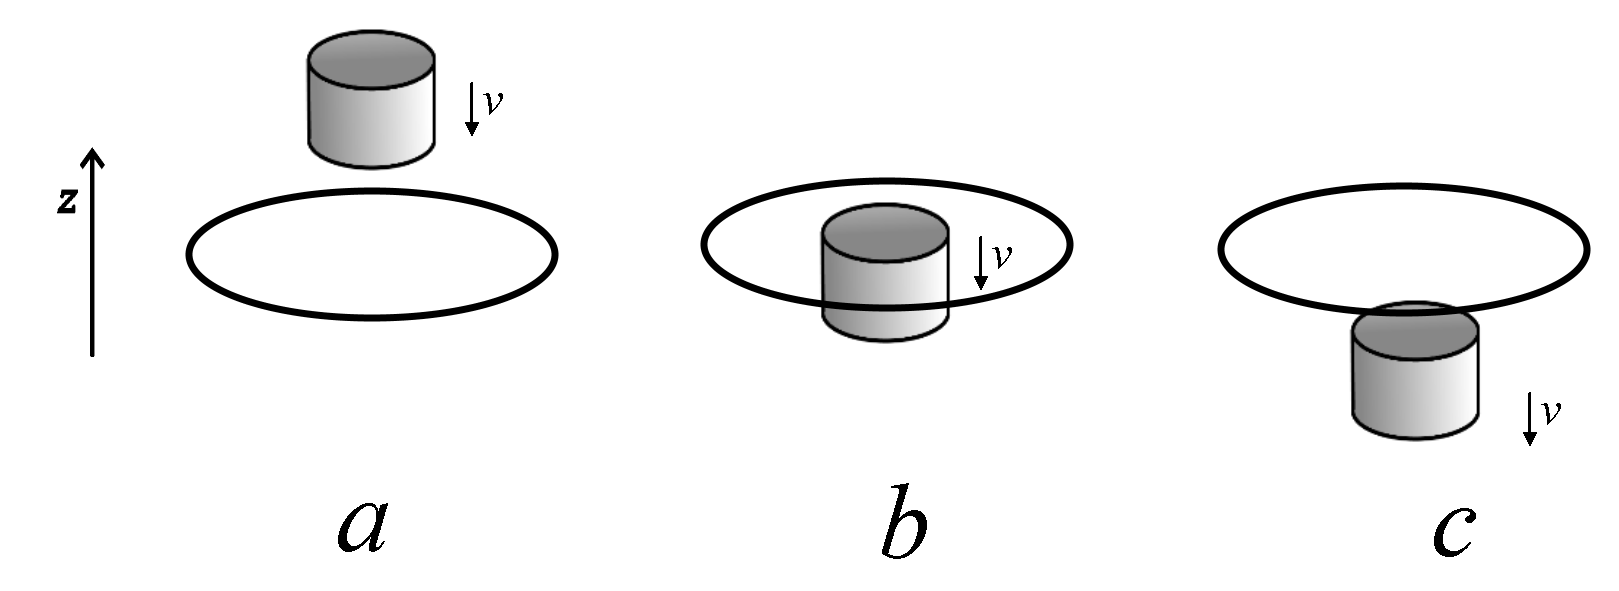
\includegraphics[width=0.9\linewidth]{figures/fallingmagnet.png}}
  \caption{
  Three different positions of the magnet falling through the ring. \label{fig:fallingmagnet}
  }
\end{figure}
%\clearpage % flush figures fig:fallingmagnet


\noindent
For each of the positions a, b and c answer the following questions:
\begin{itemize}
  \item Is current being induced in the ring? Why/why not?

  \item What is the direction of any induced current? (Use Lenz' law)

  \item How is the movement of the magnet affected and why?
\end{itemize}

\noindent
\emph{(Solution) As we release the magnet, the magnetic flux in the ring begins to change, and by Faraday's law we know that this induces an electric current in the ring.
By Biot-Savart's law this current must itself induce a magnetic field along the $z$-axis, and by Lenz' law the magnetic field must be aligned in such a way as to oppose the motion of the magnet. When the magnet is moving towards the ring (a), the induced field repels the magnet.
If the magnet is in the center of the ring (b), the momentary flux change is zero and there is no effect on the magnet. When the magnet is moving away from the ring (c), the induced field must attract the magnet.
This tells us that throughout the entire fall of the magnet (point b is just momentarily and is effectively irrelevant), the ring acts as a brake on the magnet, de-accelerating its motion.}

\section{Expanding the model}
\noindent
Now, a single metallic ring is obviously different from a lengthy metal pipe. If we wish to study the experiment at hand, we must therefore extend our model.
In order to keep the theory simple while also building on our previous discussions, we will model the pipe as a series of $N$ stacked rings, as shown in Figure~\ref{fig:ringcyl}.
The length of the pipe is $L$, and you may assume $l \ll L$.


\begin{figure}[!ht]  % fig:ringcyl
  \centerline{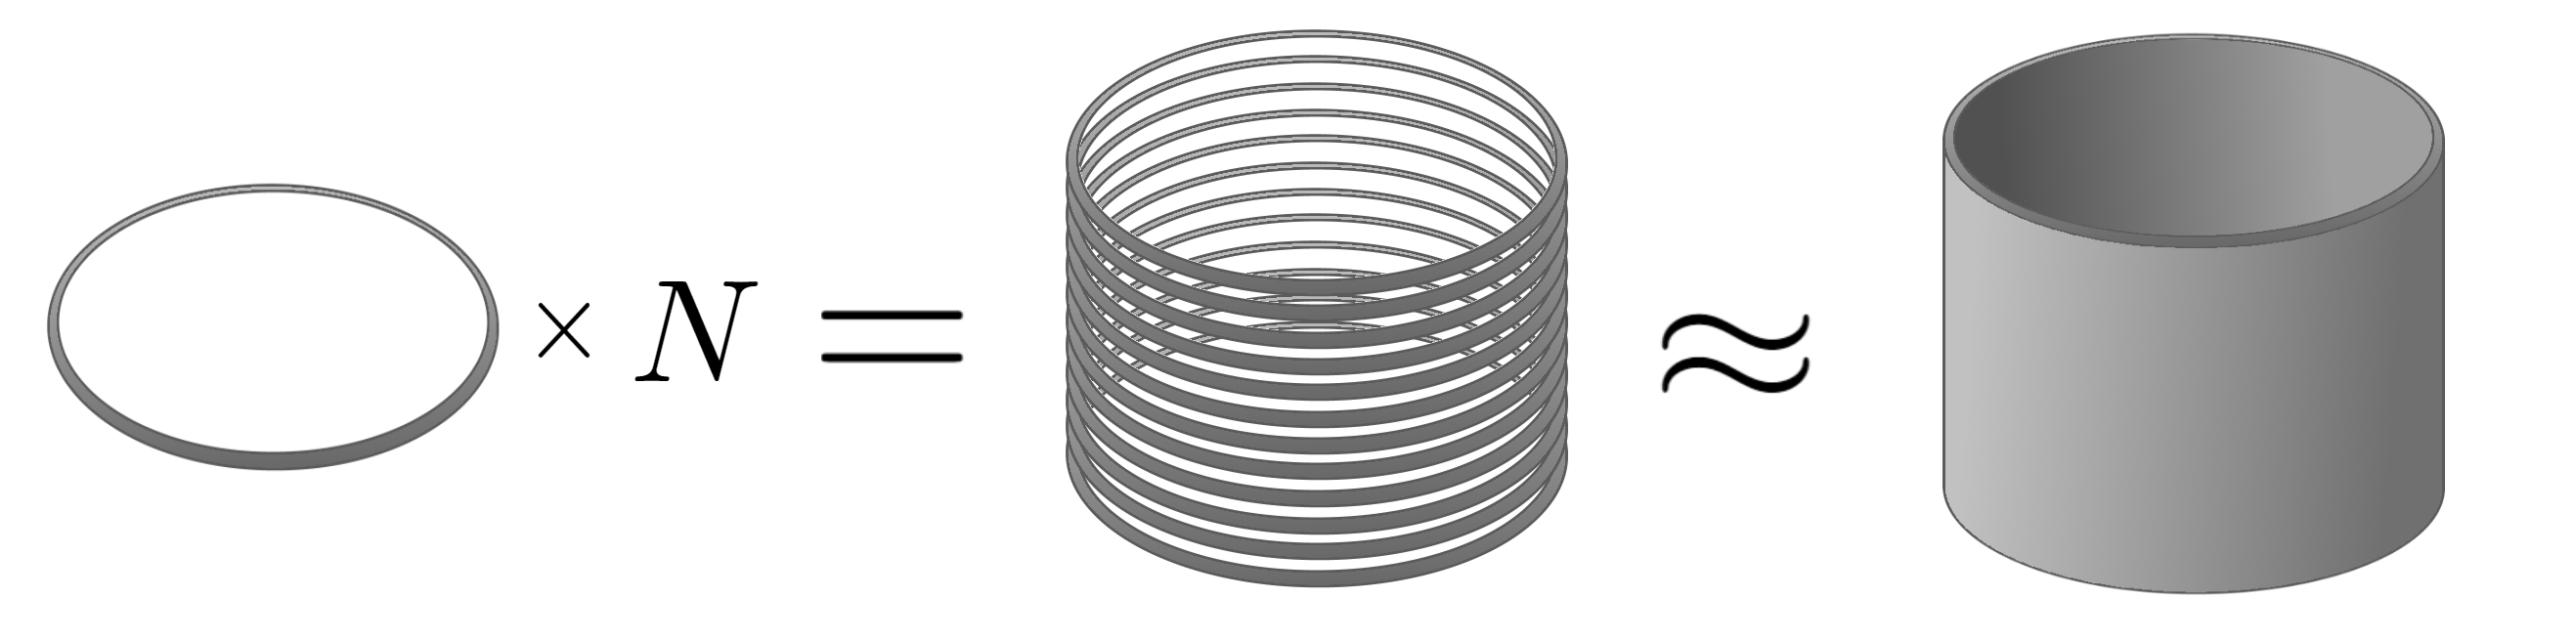
\includegraphics[width=0.9\linewidth]{figures/ringcyl.png}}
  \caption{
  \label{fig:ringcyl} Approximation of solid metal cylinder as stack of metal rings. The number of rings $N$ is arbitrarily large.
  }
\end{figure}
%\clearpage % flush figures fig:ringcyl


Ignore any mutual induction between the "rings". Knowing what you know from the last section, qualitatively answer the following exercises:
\begin{itemize}
  \item Describe the motion of the magnet inside the pipe

  \item Letting $l \ll L$ is, to some extent, effectively the same as letting $L \rightarrow \infty$. Explain why this leads to a symmetry along the $z$-axis that means that the force $F_M$ cannot depend on the vertical position of the magnet.

  \item Why may it be a reasonable approximation to assume the magnetic force on the magnet to be proportional to its velocity? In other words argue that a magnetic force on the form  $\mathbf{F_M}=k|\mathbf{v}|\mathbf{\hat{z}}$, for some constant $k>0$, is not completely unreasonable.

  \item Show that this means that the velocity \textit{must} terminate in some terminal velocity $v_T$. Like any sane physicist; neglect air resistance. (you may use some math here).
\end{itemize}

\noindent
\emph{(Solution) From the study of the magnet falling through one ring, we know that, at any point inside the pipe, the magnet will be attracted to all the "rings" above it, and repelled by all the "rings" below. This means that the magnet will be decelerated by the pipe.
In reality $F_M$ depends on the distance from each "ring" to the magnet, but if we make sure that the height of the magnet $l$ is much smaller than the length $L$ of the pipe, $l \ll L$, we may pretend that $L \rightarrow \infty$, which grants symmetry along the $z$-axis.
By "symmetry along the $z$-axis" we mean that if the pipe is infinitely long, any position on the $z$-axis must result in the same $F_M$ as any other position (there is nothing distinguishing the two situations). By this, $F_M$ can't depend on the distance to any "ring", as it would not be symmetric.
\newline An increase in velocity would mean a greater flux change through the rings, which by Lenz' law means the ring would induce a stronger magnetic field to fight the stronger flux change. Meanwhile a lower velocity would mean the rings wouldn't have to fight \textit{as} hard against the flux change.
At 0 velocity, there would of course not be any flux change, and no induced magnetic field, ergo $F_M = 0$. Due to this behavior, and the above reasoning that $F_M$ shouldn't depend on vertical position, it is not unreasonable to model as a proportionality $F_M = k v$. Because $\mathbf{F_M}$ must point towards positive $z$, we must have $k >0$.
\newline The forces acting on the magnet in the pipe are only the magnetic force, $\mathbf{F_M}=k|\mathbf{v}|\mathbf{\hat{z}}$, and gravity, $\mathbf{G} = -mg \mathbf{\hat{z}}$.
As the velocity changes, eventually the magnetic- and gravitational force will cancel each other out:
\begin{equation} \label{eq:vt}
\Sigma F = 0 = F_M + G = kv_T -mg \Rightarrow v_T = \frac{mg}{k}
\end{equation}
In our experiments we may therefore expect the velocity of the magnet to be constant when falling through the pipe.
}


\section{Experimenting}
\label{title:exp}
Hold the pipe vertically, centering the magnet above and as close to the center of the pipe as possible. Carefully drop the magnet (make sure the magnet doesn't hit the floor, as they are rather brittle!).
What do you observe? Are your results as expected from the predictions of the last section? Compare the motion of the magnet to a control-test where you drop the magnet without the pipe present.

We will now attempt to measure the terminal velocity $v_T$. We may assume that the magnet reaches its terminal velocity rather quickly (this can qualitatively be observed as well), and that the velocity is constantly $v_T$ through the entire pipe.
Using a stopwatch (or, favorably, come up with another way of measuring $v_T$ on your own!), do (at least) 5 measurements of the time $t$ it takes the magnet to fall through the entire length of the pipe $L$. Take the average of the measured times, and calculate $v_T$.
This process is shown in Figure~\ref{fig:cylindermagnets}.


\begin{figure}[!ht]  % fig:cylindermagnets
  \centerline{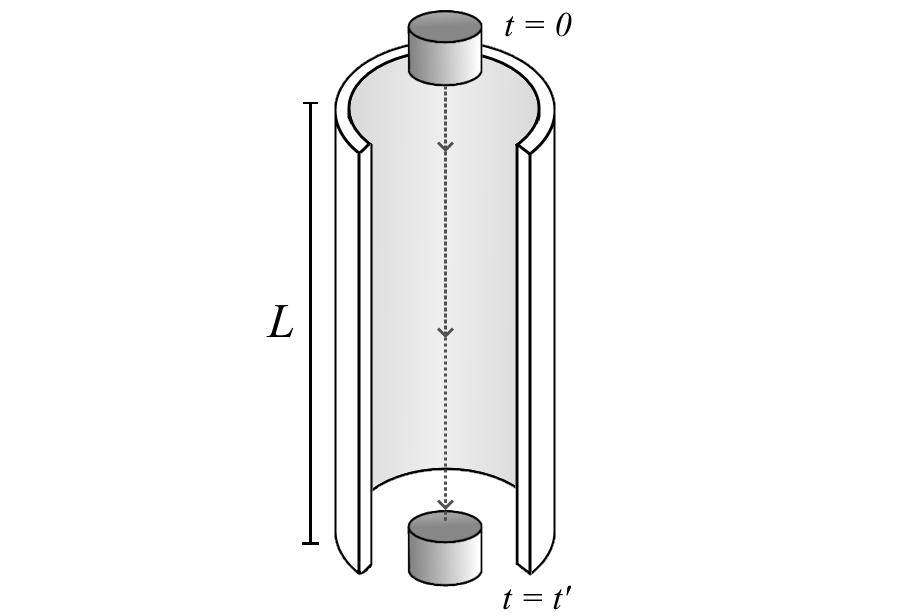
\includegraphics[width=0.9\linewidth]{figures/cylindermagnets.png}}
  \caption{
  Calculating $v_T$ by dropping the magnet through the pipe. \label{fig:cylindermagnets}
  }
\end{figure}
%\clearpage % flush figures fig:cylindermagnets


Measure the mass of the magnet\footnote{In some cases the magnet will attract metallic components within the scale, affecting the measurement. To avoid his, place something between the magnet and the scale.} $m$. Using (\ref{eq:vt}), calculate $k$. Briefly comment on its value.
Do you think your value for $k$ is very accurate? What can be done to increase its accuracy?  

\section{Measuring the resistivity of aluminum (optional)}

Provided as extra material for those of you that are curious you may find that $k$ is approximately given by
$$
k \approx \frac{45\pi^2 B_0^{2} r^{4} w\left(l^{2}+r^{2}\right)}{256 \rho R^{4}},
$$
where $B_0$ is the magnetic field measured at the center of the magnet surface, $R$ and $w$ are, respectively, the radius and width of the metal pipe. (To measure $R$ take the average of the inner and outer radii of the pipe).
Lastly, $\rho$ is the conductivity of the pipe (aluminum), which is what we wish to estimate.

There are several phone apps that lets you use your phones built-in magnetic field sensor. For both iOS and Android we recommend using "Science Journal", by Google. Use your phone to measure $B_0$,\footnote{It may be smart to research a little where within your phone the magnetic sensor is located so that you get an accurate reading on the top of the magnet. This may be done by googling something akin to "[phone model] magnetic sensor location", but on most phones it is located on the upper part of the phone, closer to the corners. You may have to spend some time tinkering with the position of the magnet relative to the phone, but ultimately $B_0$ will be the largest value you manage to read. The magnet is not strong enough to damage the electronics within your phone. However, as a precaution, please distance any magnetic cards like student ID's or bank cards while measuring $B_0$.} and use this
along with your experimental value of $v_T$ to estimate $\rho$.

Using the internet, look up the actual value of $\rho$ for aluminum. Are your values close? You should be \textit{very} happy if your answer is even within the correct power of ten, as we have done many approximations and estimations to get here.
If you wanted a more accurate measurement of $\rho$, how would you tune the experiment? What do you think is our biggest source of error?

% ------------------- end of main content ---------------

% #ifdef PREAMBLE
\end{document}
% #endif

